\documentclass[11pt, a4paper]{article}
\usepackage{fullpage}
\usepackage[USenglish]{babel}
\usepackage{graphicx} 
\usepackage[small,bf,hang]{caption2}
\usepackage{nameref}
\usepackage{hyperref}
\hypersetup{
    colorlinks,
    citecolor=black,
    filecolor=black,
    linkcolor=black,
    urlcolor=black
}

\title{Master Thesis -  Security Aspects in Virtual Networks\\ \textbf{SITREP 16}}
\author{\textbf{Laurent De Wilde} \\ Master of Science in the Applied Computer Science \\ Vrije Universiteit Brussel}
\date{April 16, 2015}

\begin{document}
\maketitle

While I was experimenting with Hyper-V, the resources on the 1U pizzaserver became sparse and I installed a second Hyper-V server. \\
This is actually the tower server with the Intel Core i7. I made a \textbf{triple boot} installation on this tower server: it now consists of the two original Windows 7 OS's and a Windows Server 2012 R2 OS on a third partition. Therefore, I had to shrink one of the two (dual boot) partitions to make space for WS2012. So the original OS's remained untouched, only a third one was added.\\ \\
However, I found it rather cumbersome to work with two seperate `Hyper-V Managers' and that's why I decided to make a small private cloud containing these two Hyper-V servers and one common interface to interact with and to manage the VM's. This interface is System Center Virtual Machine Manager 2012 R2. \\ \\
To be able to install SCVMM, I created a domain controller (VM) and also a dedicated VM that runs SQL Server 2012 and SCVMM. (FOTO NODIG) \\ \\
I will not cover all the installation and configuration details, but with al the caveats and trial and errors, it took me nearly two days to install SCVMM, to configure the domain, the storage and to get the cloud online. On the next page are some screenshots. \\ \\
While diving deeper into Hyper-V, I also discovered the ``Microsoft Security Compliance Manager'' and did some testing with it. For example, I hardened the security of one of the Windows 7 VM's using group policy objects. \\
Of course, this was not the original intention of my Master Thesis, but I really like Hyper-V and WS2012, which led to the discovering of enhanced utilities such as the Security Compliance Manager and creating a private cloud using System Center 2012 R2 Virtual Machine Manager. System Center 2012 houses other powerful tools, but I did not yet install them. \\
Maybe I could to some research and testing about private cloud security? Is there something I could test? For example, intrusion detection on private clouds, traffic capture, virtual firewalls, network access control, security of virtual disks that reside on shared storage, system hardening using SCM, \ldots.
$\;$ \\ \\
\noindent\begin{minipage}{\textwidth}
    \centering
    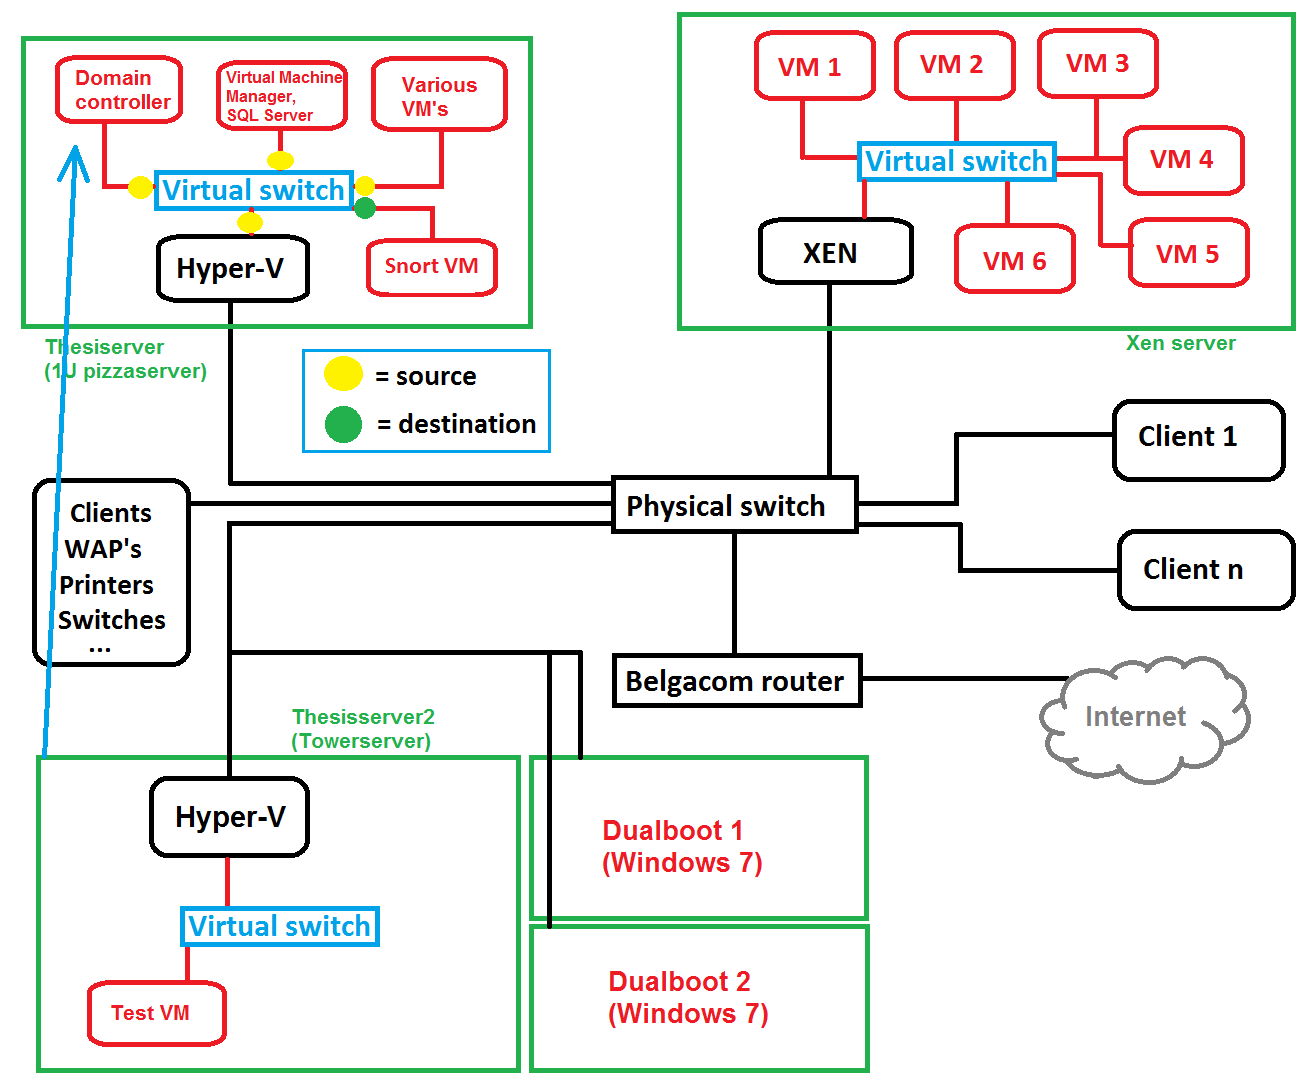
\includegraphics[width=\textwidth]{Network.png}
 \captionof{figure}{Current infrastructure.}
\end{minipage}
$\;$ \\ \\
\noindent\begin{minipage}{\textwidth}
    \centering
    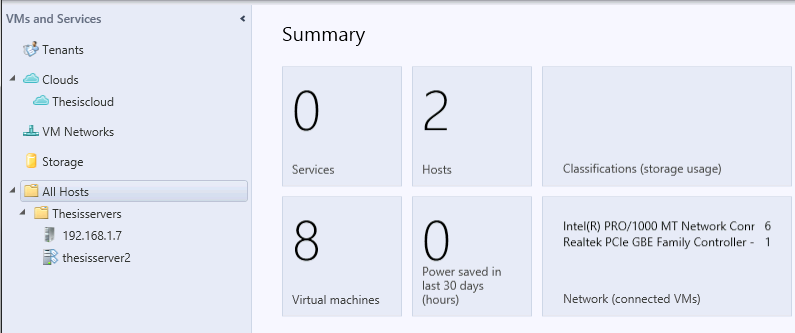
\includegraphics[width=\textwidth]{Cloud_3.png}
 \captionof{figure}{The two Hyper-V hosts with 8 VM's in total.}
\end{minipage}
$\;$ \\ \\
\noindent\begin{minipage}{\textwidth}
    \centering
    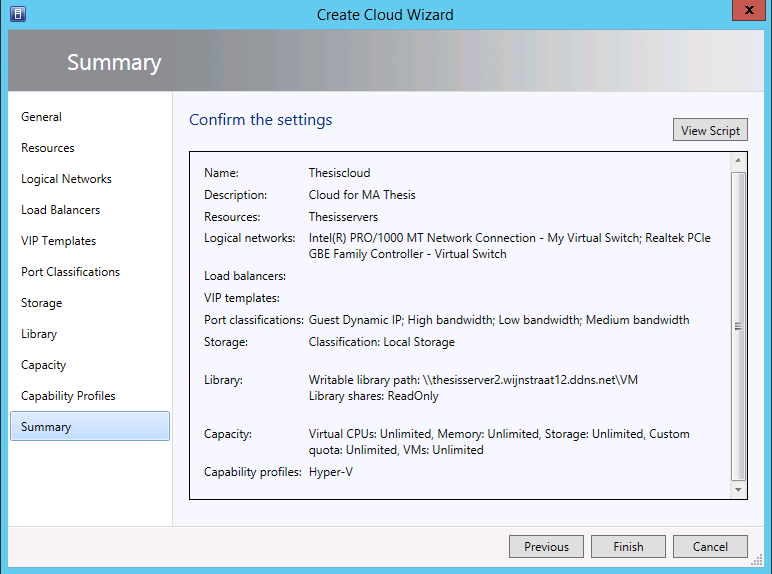
\includegraphics[width=\textwidth]{Cloud_1.png}
 \captionof{figure}{The summary of the private cloud. A library share has also been created to store the .ISO files to install the operating system on the VM's.}
\end{minipage}
$\;$ \\ \\
\noindent\begin{minipage}{\textwidth}
    \centering
    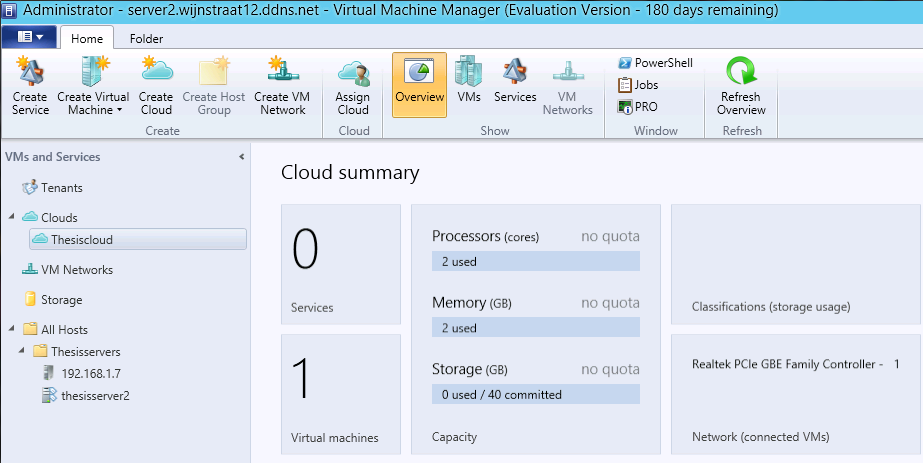
\includegraphics[width=\textwidth]{Cloud_2.png}
 \captionof{figure}{The overview of the private cloud. I created one VM in the new cloud that physically resides on ``thesisserver2'', the tower server.}
\end{minipage}
$\;$ \\ \\
\noindent\begin{minipage}{\textwidth}
    \centering
    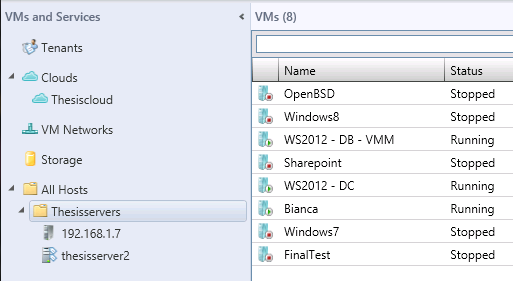
\includegraphics{Overview_1.png}
 \captionof{figure}{List of all the VM's on all the hosts and their current status.}
\end{minipage}
$\;$ \\ \\
\noindent\begin{minipage}{\textwidth}
    \centering
    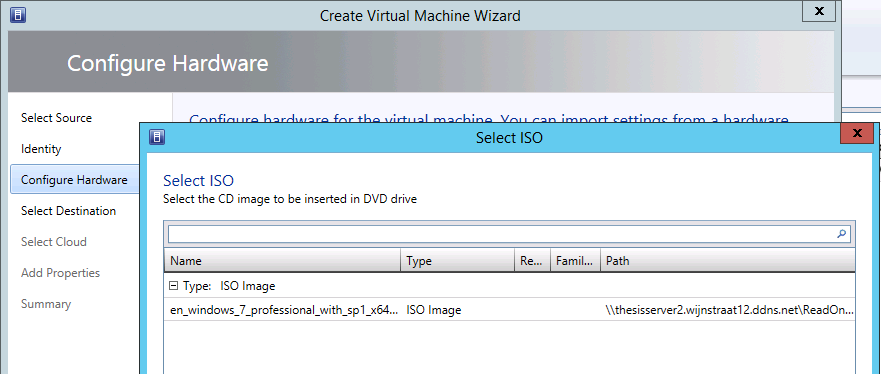
\includegraphics[width=\textwidth]{VM_1.png}
 \captionof{figure}{When adding a new VM to the cloud, an ISO image can be selected from a shared library as previously mentioned.}
\end{minipage}
$\;$ \\ \\
\noindent\begin{minipage}{\textwidth}
    \centering
    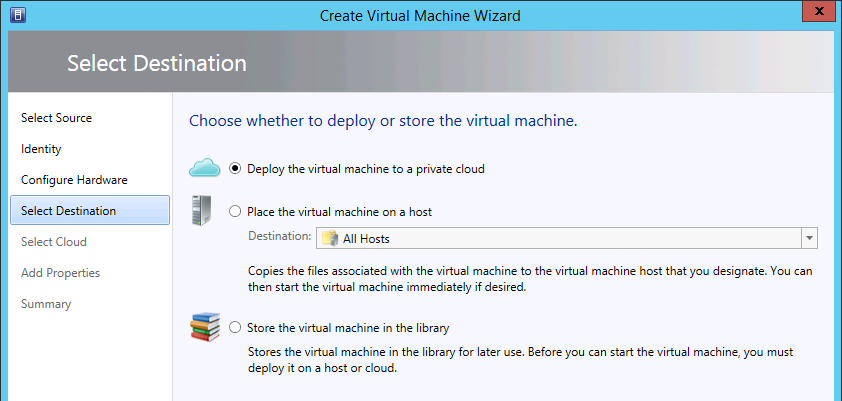
\includegraphics[width=\textwidth]{VM_2.png}
 \captionof{figure}{Deployment of the VM in the private cloud.}
\end{minipage}
$\;$ \\ \\
\noindent\begin{minipage}{\textwidth}
    \centering
    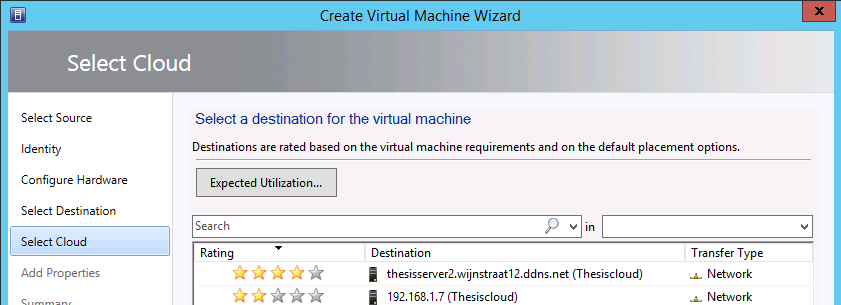
\includegraphics[width=\textwidth]{VM_3.png}
 \captionof{figure}{The most suitable place to store (run) the VM is indicated on this screen. The higher the rating, the more suitable. We opt for ``thesisserver2''.}
\end{minipage}
$\;$ \\ \\
\noindent\begin{minipage}{\textwidth}
    \centering
    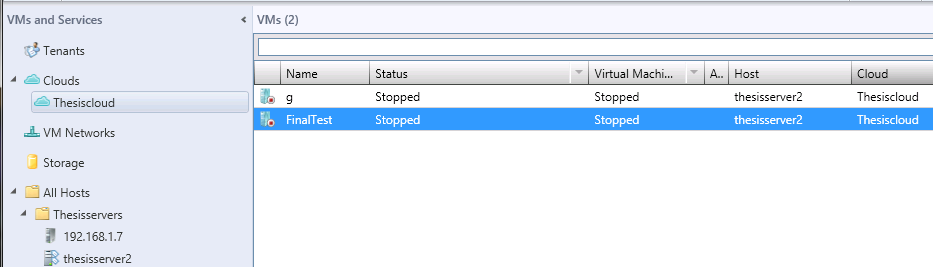
\includegraphics[width=\textwidth]{VM_4.png}
 \captionof{figure}{The VM is deployed in the cloud\ldots}
\end{minipage}
$\;$ \\ \\
\noindent\begin{minipage}{\textwidth}
    \centering
    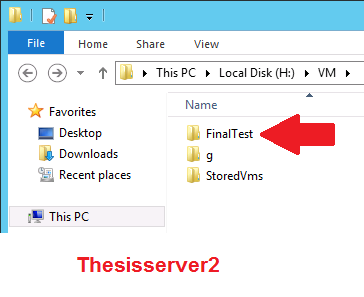
\includegraphics{VM_5.png}
 \captionof{figure}{\ldots and stored physically on the tower server on the default location that has been specified when I configured the private cloud.}
\end{minipage}
$\;$ \\ \\
\noindent\begin{minipage}{\textwidth}
    \centering
    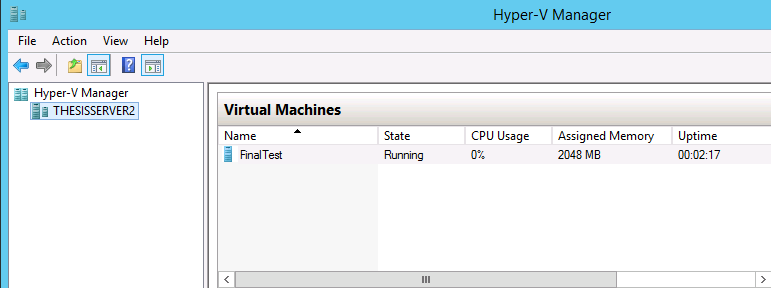
\includegraphics[width=\textwidth]{VM_6.png}
 \captionof{figure}{And indeed, the VM is listed in Hyper-V Manager of the target server \ldots}
\end{minipage}
$\;$ \\ \\
\noindent\begin{minipage}{\textwidth}
    \centering
    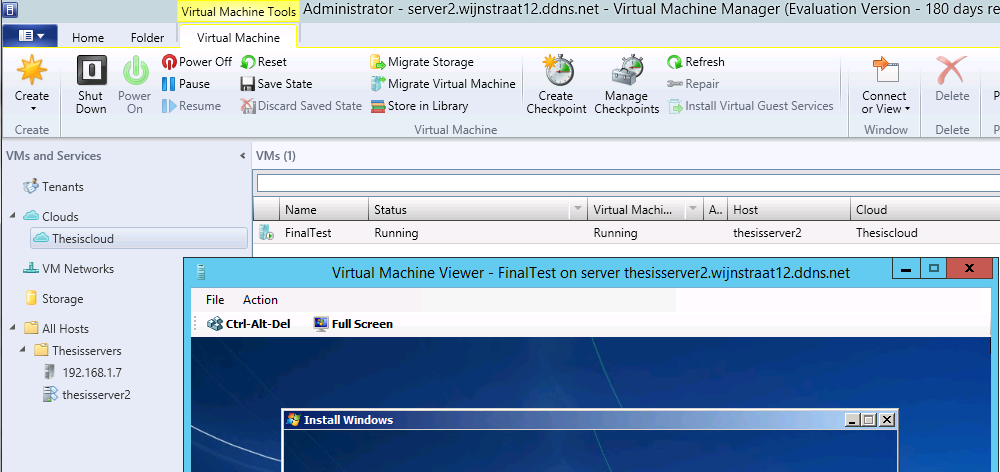
\includegraphics[width=\textwidth]{VM_7.png}
 \captionof{figure}{\ldots but now I can control all the VM's from a single management console, which makes it more efficient. I must say, SCVMM is a very handy and powerful tool. I have never used it before, but will certainly continue using it.}
\end{minipage}
$\;$ \\ \\
\noindent\begin{minipage}{\textwidth}
    \centering
    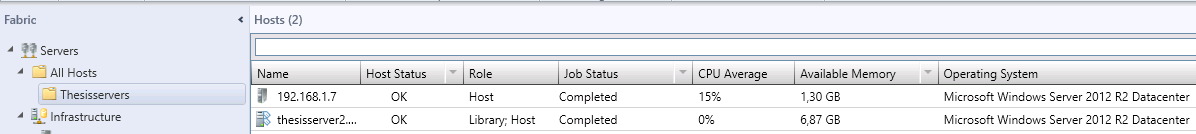
\includegraphics[width=\textwidth]{Hosts_1.png}
 \captionof{figure}{A short overview of the hosts.}
\end{minipage}
$\;$ \\ \\
\noindent\begin{minipage}{\textwidth}
    \centering
    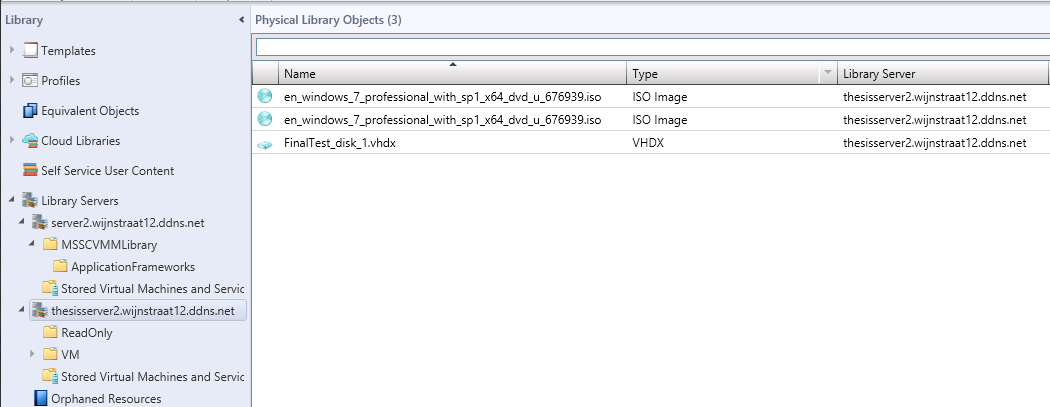
\includegraphics[width=\textwidth]{Hosts_2.png}
 \captionof{figure}{The physical objects stored on the library servers.}
\end{minipage}


\section*{Planning}



\section*{Problems}



\section*{Issues}



\section*{Assistance}

Of course, this was not the original intention of my Master Thesis, but I really like Hyper-V and WS2012, which led to the discovering of enhanced utilities such as the Security Compliance Manager and creating a private cloud using System Center 2012 R2 Virtual Machine Manager. System Center 2012 houses other powerful tools, but I did not yet install them. \\
Maybe I could to some research and testing about private cloud security? Is there something I could test? For example, intrusion detection on private clouds, traffic capture, virtual firewalls, network access control, security of virtual disks that reside on shared storage, system hardening using SCM, \ldots.


\end{document}